\section{Introduction}
In this master thesis we will study how to implement an  electronic voting scheme application based on some tools from cryptography where the most important tool is the Publicly Verifiable Secret Sharing (PVSS) protocol. The main paper for this protocol will be Berry Schoenmakers paper "A Simple Publicly Verifiable Secret Sharing Scheme and its Application to Electronic Voting" \cite{Schoenmakers1999}. \\\\
\noindent
Secret sharing is a tool used in the PVSS protocol. Secret sharing is a way of distributing a secret among several servers. Secret sharing is where a dealer has a secret. The dealer shares pieces of the secret to each of the players. If there are a large number of players they will be able to reconstruct the secret. More technically the idea is to hide a secret inside of a polynomial so that given certain partial information of the polynomial we can recover the secret that was hidden in it.\\\\
\noindent
A Multiparty computation protocol (MPC) is a protocol which uses secret sharing and allows several parties to compute some function on some private inputs, in such a way that they learn the result but not the inputs from the other players. MPC is not using conventional methods, where some commonly trusted party, could gather sensitive information. The figure to the left is showing a judge who all participants trust to give their secret inputs. The trusted party can then compute the outcome of the process, for instance the sum of all inputs, and reveal the output. The right figure is how an equivalent MPC would work. Here there is no trusted party, but by using multiparty computation they can still achieve the same level of secrecy, but without having to trust someone.
 
\begin{center}
     \makebox[\textwidth]{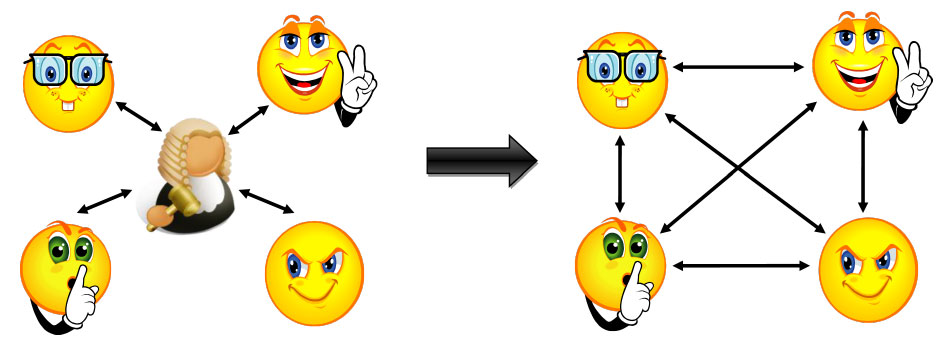
\includegraphics[scale=0.35]{MPC.jpg}}
\end{center}

\noindent
This leads to a core observation namely that without a trusted party the ability to validate the input the MPC protocol relies on the participants honesty. 
The PVSS protocol used in this thesis proposes a solution to this problem. The idea is that not only can the participants verify their own shares, but that anybody can verify the correctness of the transmitted data.